\documentclass[12pt,letterpaper]{article}
\usepackage[latin1]{inputenc}
\usepackage[spanish]{babel}
\usepackage{amsmath}
\usepackage{amsfonts}
\usepackage{amssymb}
\usepackage{graphicx}
\usepackage[hidelinks]{hyperref}
\usepackage{color}
\usepackage[left=2cm,right=2cm,top=2cm,bottom=2cm]{geometry}
\author{M�rquez M�rquez Amairani Ivette}
\begin{document}
\begin{center}
\textbf{\huge{Universidad Politecnica de la Zona\\[0.5cm] Metropolitana de Guadalajara}}

\includegraphics[width=0.65\textwidth]{Imagenes/UPCDLZMDG5783-logo.png}\\[2cm] 
\end{center}
\vspace{0.1cm}
{\large\textbf{Evidencia:} 1.5 Caracteristicas de los convertidores de potencia CA-CD, CD-CA, CA-CA Y CD-CD\\[0.2cm]\textbf{Alumna:} M�rquez M�rquez Amairani Ivette\\[0.2cm]\textbf{Profesor:} Mor�n Garabito Carlos Enrique\\[0.2cm]\textbf{Carrera:} Ing.Mecatronica\\[0.2cm]\textbf{Grupo:} 4�B\\[0.2cm]\textbf{Fecha de entrega:} 17 de Septiembre del 2019}\\[0.2cm]\\

\vspace{10cm}
\begin{center}
\textbf{Caracteristicas de los convertidores de potencia CA-CD, CD-CA, CA-CA Y CD-CD}\\[0.3cm]
\end{center}
Un convertidor de CA/CC puente de diodos genera un factor de potencia muy bajo, al sumarle un convertidor CC/CC se obtiene una corriente regulada, sin embargo, la corriente de entrada no se encuentra en fase con el voltaje y tampoco es senoidal. Una topolog�a como �sta no cumple los requerimientos de un alto factor de potencia.\\


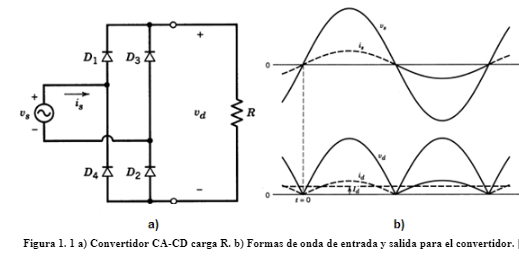
\includegraphics[scale=1]{Imagenes/Captura.PNG}\\ 


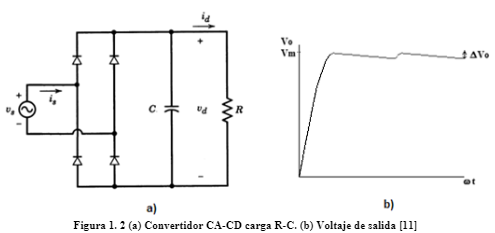
\includegraphics[scale=1]{Imagenes/Captura_1.PNG}\\

\vspace{0.2cm}

Por esta raz�n se sugiere el dise�o de un circuito que entregue un voltaje en CC regulado, dicha estructura debe cumplir las condiciones ideales para el mejoramiento del factor de potencia como son una corriente de entrada en fase con el voltaje de la fuente, la forma senoidal que debe tener el voltaje y la corriente. Tambi�n se debe considerar que sera la corriente que soporten los dispositivos y el an�lisis de la potencia entregada en la carga con respecto a la potencia requerida en la fuente para conocer la eficiencia de la topolog�a.\\

\vspace{0.2cm}

{\large\textbf{Bibliograf�a}}
\begin{center}
\emph{Blanco.S(Marzo 2017). Capitulo 1. Convertidores de Potencia - PDF.}Obtenido de:
\textcolor{blue}{https://docplayer.es/14077510-Capitulo-i-convertidores-de-ca-cd-y-cd-ca.html}\\[0.2cm]
\end{center}

\end{document}